%!TEX root = ../my_thesis.tex
\chapter{Décodeurs polaires déclenchés par transport} % (fold)
\label{chap:tta}

\vspace*{\fill}
\minitocTITI
\vspace*{\fill}
\newpage

\section*{Introduction}

\section{Transport Triggered Architectures}
\subsection{Principes}
\begin{figure}
\centering
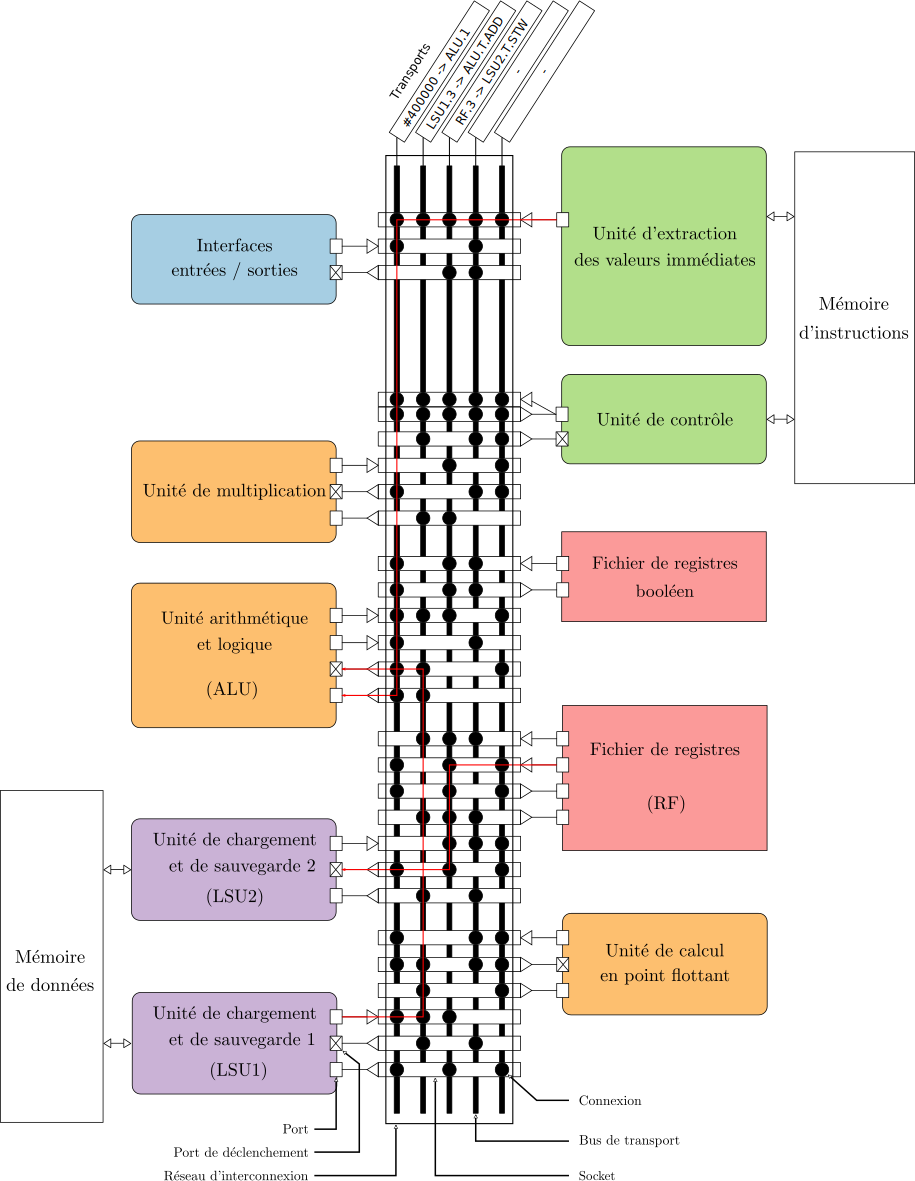
\includegraphics[scale=0.6]{main/ch4_fig/archi_tta}
\end{figure}
\subsection{Environnement TCE}

\section{Transport Triggered Polar Decoders}

\subsection{Architecture du décodeur SC}
\subsection{Description logicielle}
\subsection{Implémentation de l'algorithme SCAN}

\section{Un flot de conception complet}

\subsection{Génération des vecteurs de tests}
\subsection{Cycles de conception}

\section{Expérimentations et mesures}

\subsection{TT-SC}
\subsection{TT-SCAN}


\section*{Conclusion}


